\documentclass[11pt
  , a4paper
  , article
  , oneside
  %  , twoside
  , showtrims
 % , draft
]{memoir}

\usepackage{essdocs}
\usepackage[numbers]{natbib}
\usepackage[autostyle]{csquotes}

%% \usepackage{epstopdf}
%% \usepackage[pdf]{pstricks}
%% \usepackage{graphicx}

\setsecnumdepth{subsection}

\begin{document}
%\frontmatter
%% ESS Document Description
%%
\essdocdesc{Engineering Manual}

%% ESS Document Number
%%
\essdocnum{ESS-XXXXXXXX}

%% Date
%%
\date{\today}

%% ESS Document Revision Number
%%
\essdocrev{0.2}

%% ESS Document State
%%
\essdocstate{Early Draft}

%% ESS Document Classification
%%
\essdocclass{ESS Use Only}

%% Document Title
%%
\title{ICS Engineering Manual}
\subtitle{for MRF MTCA-EVR-300}
%% Document Author(s), if more than one author,
%% use \newline instead of \\ or \linebreak in order to seperate them
\author{Javier Cereijo Garcia \newline Jeong Han Lee }

%% Document Reviewer(s) if more than one reviewer,
%% use \newline instead of \\ or \linebreak in order to seperate them
%\reviewer{Timo Korhonen (Chief Engineer) \newline Timo Korhonen (Chief Engineer)}
\reviewer{TBD}
%% Document Owner(s) if more than one owner,
%% use \newline instead of \\ or \linebreak in order to seperate them
\owner{ICS}

%% Document Approver(s) if more than one approver,
%% use \newline instead of \\ or \linebreak in order to seperate them
\approver{ICS}

\showtrimson

\esstitle
\newpage
\tableofcontents
\newpage

%\mainmatter


%%% Actual Document Start at below
\chapter{Overview}
At European Spallation Source (ESS), Integrated Control System (ICS) does use the Micro Research Finland (MRF) Timing System{\footnote{\url{http://www.mrf.fi/}}} as its timing system of the ESS site. The consistent and up-to-date engineering manual is essential for the ESS Timing system.

\section{Scope}
\begin{itemize}
\item This document identifies one of the MRF Timing Event Receivers (EVR) that needs to be configured for an ESS subsystem that needs synchronous frequencies, trigger signals and sequences of events \cite{MRFEVENTSYSTEMDC}.
\item This document provides the generic description of the MRF MTCA-EVR-300 and its interface board (IFB-300). In addition, it affords the minimal, essential, and generic information for the system configuration.  
\item The purpose of this document is to describe the engineering procedure and troubleshooting about how the MRF MTCA-EVR-300 board will be integrated in cooperation with the ESS EPICS Environment (EEE).
\item This document attempts to maintain consistency with existing ESS Timing system hardware as far as possible. 
\end{itemize}
\textbf{Note that this is a very early draft document and should be updated as development progresses.}

\section{Target Audience}
This document is targeted to ICS engineers and technical stakeholders of the ESS timing system. It is assumed that the target audience has a technical background in the MRF Timing System, the EPICS development, and a Linux environment.

\chapter{System Description}
MRF Technical Reference \citep[see][p45]{MRFEVENTSYSTEMDC} explained Event Receivers and wrote :
\blockquote{\textit{Event Receivers decode timing events and signals from an optical event stream transmitted by an Event Generator. Events and signals are received at predefined rate the event clock that is usually divided down from an accelerators main RF reference. The event receivers lock to the phase event clock of the Event Generator and are thus phase locked to the RF reference. Event Receivers convert event codes transmitted by an Event Generator to hardware outputs. They can also generate software interrupts and store the event codes with globally distributed timestamps into FIFO memory to be read by a CPU.}}

ICS uses and will use the following different types of EVR :
\begin{itemize}
\item MTCA-EVR-300
\item PCIe-EVR-300DC
\end{itemize}

The scope of this document is to cover MTCA-EVR-300 board.


\section{MTCA-EVR-300}
Figure~\ref{fig:mtca-evr300} shows the rough physical dimensions $181\times 148~\mathrm{mm}{}^2$ of the MTCA-EVR-300 card.

\begin{figure}[!htb]
  \centering
  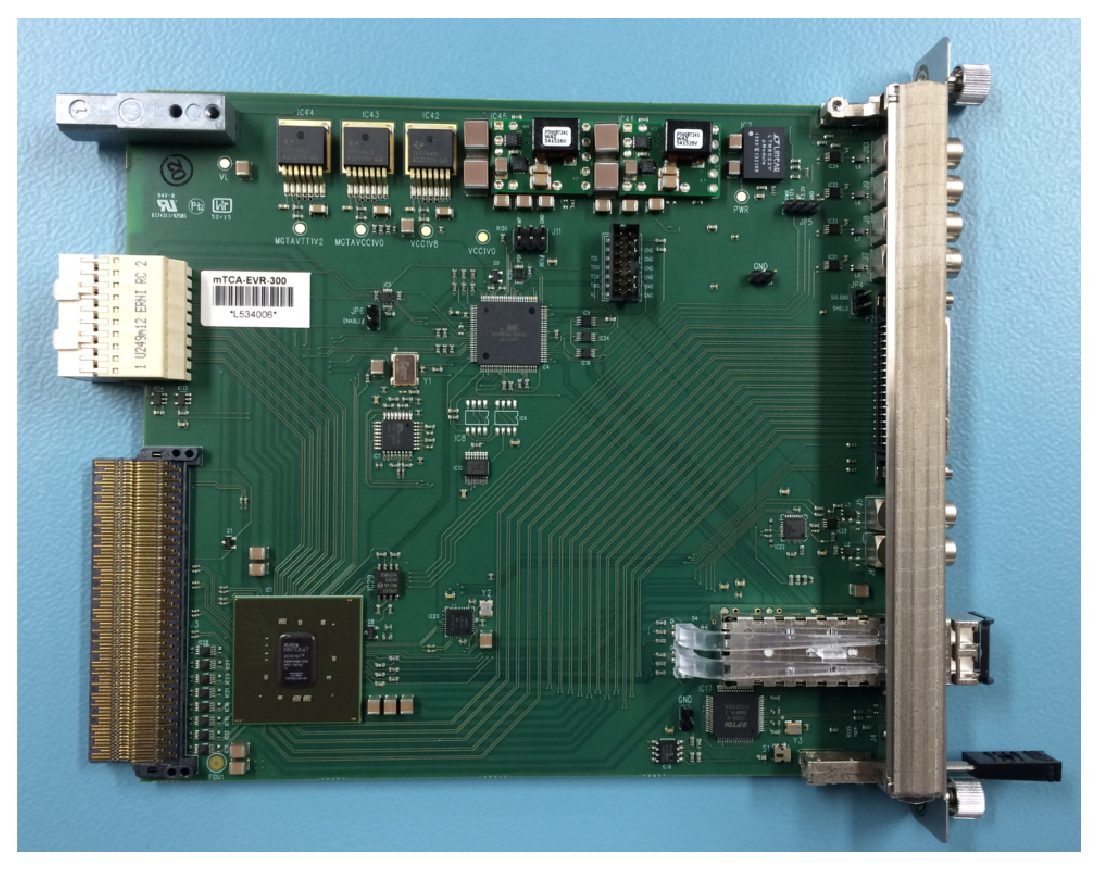
\includegraphics[width=0.99\textwidth]{./pictures/mtca_evr_300.eps}
  \caption{
    MRF MTCA-EVR-300 board.
  }
  \label{fig:mtca-evr300}   
\end{figure}


The MTCA-EVR-300  has a SFP transceiver as an input from EVG and several outputs: 4 front panel outputs, 16 front universal outputs (through the IFB-300 extension board) and 40 rear outputs. The initial 32 rear outputs map to the RTM connector, the last 8 rear outputs map to the MTCA backplane. The 16 front universal outputs are implemented through a micro-SCSI type connector for an interface board IFB-300. The IFB-300 has eight Universal I/O slots, shown in Figure~\ref{fig:ifb-300}. With different type of MRF Universal I/O modules, each slot can be used as an unique trigger or event signal source.

\begin{figure}[!htb]
  \centering
  \includegraphics{./pictures/ifb-300.eps}
  \caption{
    MRF Interface Board IFB 300 Front Panel \cite{MRFEVENTSYSTEMDC}.
  }
  \label{fig:ifb-300}   
\end{figure}


\clearpage

\chapter{System Environment}
Before describing the engineering procedure for an EEE integration of the MRF MTCA-EVR-300 board, it is mandatory to have proper system environment that consists of specific hardware and software lists. Here we will show the hardware and software lists, their block diagrams, and their setup in the ICS lab at ESS. The information shown in this chapter is used in the ICS Lab at ESS.


\section{Hardware}
Table~\ref{table:hwlist} shows the hardware list and its environment. Here, \texttt{TAG} is used as the prefix of the ICS internal inventory system in order to track it down.
\begin{table}[!hb]
  \centering
  \begin{tabular}{l|l|l}
    \toprule
    Hardware                        & Info                                               & Serial Number \\\midrule
    MRF MTCA-EVR-300                & \texttt{ICS TAG-???}                               & ???       \\\midrule
    NAT-MCH-PHYS                    & \texttt{ICS TAG-???}                               & ???    \\\midrule
    Concurrent Technologies AMC CPU & \texttt{ICS TAG-???}, hostname: ???                & ???     \\\midrule
    ELMA MTCA crate 12 slots, 9U    & \texttt{ICS TAG-???}                               & ???      \\\midrule
    Wiener power supply unit 1000W  & \texttt{ICS TAG-???}                               & ???       \\\midrule
    Ethernet cables                 &                                                    & ???              \\\bottomrule
  \end{tabular}
  \caption[]{Hardware List and Its Environment.}
  \label{table:hwlist}
\end{table}


% Figure~\ref{fig:diagram} shows the physical hardware setup and 
Figure~\ref{fig:mtca-hw-setup} shows the MTCA-EVR-300 setup in the lab. From left to right, the power supply, MCH, CPU, MTCA-EVR-300 and Struck SIS8300 (not used in this document).
\begin{figure}[!b]
  \centering
  \includegraphics[width=0.8\textwidth]{./pictures/mtca-hw-setup.eps}
  \caption{Hardware Setup in the ICS lab.}
  \label{fig:mtca-hw-setup}   
\end{figure}


\clearpage
\section{Software}
Table~\ref{table:swlist} shows the Software list and its environment. It is mandatory to check the kernel version, and the mrf kernel module version. Since the mrfioc2 is dependent upon devLibs2 EEE internally, an end-user is unnecessary to check its version explicitly. 
\begin{table}[!htb]
  \centering
  \begin{tabular}{l|l}
    \toprule
    Item               & Version Info.                                                       \\\midrule
    CentOS Linux       & \texttt{7.1.1503}                                                   \\\midrule
    Kernel             & \texttt{3.10.0-229.7.2.el7.x86\_64}                                 \\\midrule
    mrf kernel module  & version : \texttt{1} / srcversion \texttt{9E849DD3775C8555B8B88BF}  \\\midrule
    EEE                & \texttt{1.8.2}                                                      \\\midrule
    EPICS Base         & \texttt{3.15.4}                                                     \\\midrule
    mrfioc2            & EEE module ver. \texttt{2.7.13}                                     \\\midrule
    devLib2            & EEE module ver. \texttt{2.7.0}                                      \\\bottomrule
  \end{tabular}
  \caption[]{Software and its version information.}
  \label{table:swlist}
\end{table}

\section{EVR Firmware}
Table~\ref{table:fwinfo} shows EVR FPGA Firmware Version Register.

\begin{table}[!htb]
  \centering
  \begin{tabular}{p{0.3\linewidth}|c|l}
    \toprule
    EVR FPGA Firmware Version Register            & \multicolumn{2}{c}{\texttt{0x18000207}}             \\\midrule
    Board Type      & EVR                         &  \texttt{0x}\underline{\textbf{1}}\texttt{8000207}  \\\midrule
    Form Factor     & mTCA.4                      &  \texttt{0x1}\underline{\textbf{8}}\texttt{000207}  \\\midrule
    EVR Firmware ID & Delay Compensation Firmware &  \texttt{0x1800}\underline{\textbf{02}}\texttt{07}  \\\midrule
    EVR Revision ID & 7                           &  \texttt{0x180002}\underline{\textbf{07}}           \\\bottomrule
  \end{tabular}
  \caption[]{EVR FPGA Firmware Version Register in Reference \citep[see][p66]{MRFEVENTSYSTEMDC}.}
  \label{table:fwinfo}
\end{table}


\clearpage
\chapter{Engineering Procedure}
This chapter provides the minimal information to configure the EVR board properly. 

\section{System Installation} 
Figure~\ref{fig:mtca-hw-setup} shows the glimpse of what system might be like in a Lab. \textbf{Note that the cable between the mTCA-EVR-300DC and IFB-300 (not shown in the figure) should be connected, disconnected, or both only when powered down}. Please see the detail information in Reference \citep[][p54]{MRFEVENTSYSTEMDC}.

It is assumed that the MTCA-EVR-300 is installed in a crate with a CPU running CentOS 7.1 with EEE.
  
\section{mTCA-EVR-300 Board Identification}

\subsection{Fixing PCI IDs}
The PCI ID list does not include the MRF products. It can be updated as follows:
\begin{itemize}
\item Cloning the sort of ESS customized PCI.IDS db:
\begin{lstlisting}[style=termstyle]
iocuser@localhost: ics_gitsrc$ git clone https://github.com/jeonghanlee/pciids
\end{lstlisting}
\item Replace the pci.ids file:
\begin{lstlisting}[style=termstyle]
iocuser@localhost: pciids (master)$ bash replace-pciids.bash 
centos was determined.
[sudo] password for iocuser: 
\end{lstlisting}
\item Check MRF products by the ventor's id (1a3e):
\begin{lstlisting}[style=termstyle]
iocuser@localhost: pciids (master)$ lspci -nmmn | grep -E "\<(1a3e)"
05:00.0 "Signal processing controller [1180]" "Xilinx Corporation [10ee]" "XILINX PCI DEVICE [7011]" "Micro-Research Finland Oy [1a3e]" "MTCA Event Receiver 300 [132c]"
\end{lstlisting}
\end{itemize}

\subsection{Setting up MRF environment}
The MTCA-EVR-300 needs a kernel module to work. It can be installed by simply running a script. Do the following:
\begin{itemize}
\item Get the script:
\begin{lstlisting}[style=termstyle]
iocuser@localhost: ics_gitsrc$ git clone https://github.com/icshwi/icsem_scripts
\end{lstlisting}
\item Chech the information:
\begin{lstlisting}[style=termstyle]
 iocuser@localhost: icsem_scripts (master)$ bash mrf_setup.bash 

usage: mrf_setup.bash <arg>

          <arg> : info

          show  : show the found mrf boards information 

          pac   : mrf package from ESS (do not use now) 
                  We are working on this.... 

          src   : compile kernel module from git repository 
                  https://bitbucket.org/europeanspallationsource/m-epics-mrfioc2
                  tag name : ess-2-7

          rule : put only the mrf kernel and udev rules 

iocuser@localhost: icsem_scripts (master)$ bash mrf_setup.bash show

We've found the MRF boards as follows:
--------------------------------------
05:00.0 "Signal processing controller [1180]" "Xilinx Corporation [10ee]" "XILINX PCI DEVICE [7011]" "Micro-Research Finland Oy [1a3e]" "MTCA Event Receiver 300 [132c]"
\end{lstlisting}
\item Install the kernel module:
\begin{lstlisting}[style=termstyle]
iocuser@localhost: icsem_scripts (master)$ bash mrf_setup.bash src
[sudo] password for iocuser: 

>>>> You are entering in  : git_compile_mrf

>>>> You are entering in  : git_clone
No git source repository in the expected location /home/iocuser/ics_gitsrc/icsem_scripts/m-epics-mrfioc2
Cloning into '/home/iocuser/ics_gitsrc/icsem_scripts/m-epics-mrfioc2'...
remote: Counting objects: 460, done.
remote: Compressing objects: 100% (364/364), done.
remote: Total 460 (delta 156), reused 246 (delta 84)
Receiving objects: 100% (460/460), 1.76 MiB | 1.34 MiB/s, done.
Resolving deltas: 100% (156/156), done.

<<<< You are leaving from : git_clone
~/ics_gitsrc/icsem_scripts/m-epics-mrfioc2/mrmShared/linux ~/ics_gitsrc/icsem_scripts
make -C /lib/modules/3.10.0-229.7.2.el7.x86_64/build M=/home/iocuser/ics_gitsrc/icsem_scripts/m-epics-mrfioc2/mrmShared/linux modules
make[1]: Entering directory `/usr/src/kernels/3.10.0-229.7.2.el7.x86_64'
  CC [M]  /home/iocuser/ics_gitsrc/icsem_scripts/m-epics-mrfioc2/mrmShared/linux/uio_mrf.o
  CC [M]  /home/iocuser/ics_gitsrc/icsem_scripts/m-epics-mrfioc2/mrmShared/linux/jtag_mrf.o
  LD [M]  /home/iocuser/ics_gitsrc/icsem_scripts/m-epics-mrfioc2/mrmShared/linux/mrf.o
  Building modules, stage 2.
  MODPOST 1 modules
  CC      /home/iocuser/ics_gitsrc/icsem_scripts/m-epics-mrfioc2/mrmShared/linux/mrf.mod.o
  LD [M]  /home/iocuser/ics_gitsrc/icsem_scripts/m-epics-mrfioc2/mrmShared/linux/mrf.ko
make[1]: Leaving directory `/usr/src/kernels/3.10.0-229.7.2.el7.x86_64'
make -C /lib/modules/3.10.0-229.7.2.el7.x86_64/build M=/home/iocuser/ics_gitsrc/icsem_scripts/m-epics-mrfioc2/mrmShared/linux modules_install
make[1]: Entering directory `/usr/src/kernels/3.10.0-229.7.2.el7.x86_64'
  INSTALL /home/iocuser/ics_gitsrc/icsem_scripts/m-epics-mrfioc2/mrmShared/linux/mrf.ko
Can't read private key
  DEPMOD  3.10.0-229.7.2.el7.x86_64
make[1]: Leaving directory `/usr/src/kernels/3.10.0-229.7.2.el7.x86_64'
make -C /lib/modules/3.10.0-229.7.2.el7.x86_64/build M=/home/iocuser/ics_gitsrc/icsem_scripts/m-epics-mrfioc2/mrmShared/linux clean
make[1]: Entering directory `/usr/src/kernels/3.10.0-229.7.2.el7.x86_64'
  CLEAN   /home/iocuser/ics_gitsrc/icsem_scripts/m-epics-mrfioc2/mrmShared/linux/.tmp_versions
  CLEAN   /home/iocuser/ics_gitsrc/icsem_scripts/m-epics-mrfioc2/mrmShared/linux/Module.symvers
make[1]: Leaving directory `/usr/src/kernels/3.10.0-229.7.2.el7.x86_64'
~/ics_gitsrc/icsem_scripts

<<<< You are leaving from : git_compile_mrf

>>>> You are entering in  : modprobe_mrf

<<<< You are leaving from : modprobe_mrf

>>>> You are entering in  : put_mrf_rule
Put the rule : mrf in /etc/modules-load.d/mrf.conf to load the mrf module at boot time.
mrf
<<<< You are leaving from : put_mrf_rule

>>>> You are entering in  : put_udev_rule
Put the rule : KERNEL=="uio*", ATTR{name}=="mrf-pci", MODE="0666" in /etc/udev/rules.d/99-mrfioc2.rules to be accessible via an user.
KERNEL=="uio*", ATTR{name}=="mrf-pci", MODE="0666"
<<<< You are leaving from : put_udev_rule
 0: SCRPIT      : /home/iocuser/ics_gitsrc/icsem_scripts/mrf_setup.bash
 1: SCRIPT NAME : mrf_setup.bash
 2: SCRIPT TOP  : /home/iocuser/ics_gitsrc/icsem_scripts
 3: LOGDATE     : 2017Feb06-1435-02CET
 4: filename:       /lib/modules/3.10.0-229.7.2.el7.x86_64/extra/mrf.ko
author:         Michael Davidsaver <mdavidsaver@bnl.gov>
version:        1
license:        GPL v2
rhelversion:    7.1
srcversion:     9E849DD3775C8555B8B88BF
depends:        parport,uio
vermagic:       3.10.0-229.7.2.el7.x86_64 SMP mod_unload modversions 
parm:           cable:Name of JTAG parallel port cable to emulate (charp)
parm:           interfaceversion:User space interface version (int)
 5: mrf                    17592  0 
uio                    19259  1 mrf
parport                42348  1 mrf
\end{lstlisting}
\item Check kernel module information:
\begin{lstlisting}[style=termstyle]
iocuser@localhost: icsem_scripts (master)$ lsmod |grep mrf
mrf                    17592  0 
uio                    19259  1 mrf
parport                42348  1 mrf
iocuser@localhost: icsem_scripts (master)$ modinfo mrf
filename:       /lib/modules/3.10.0-229.7.2.el7.x86_64/extra/mrf.ko
author:         Michael Davidsaver <mdavidsaver@bnl.gov>
version:        1
license:        GPL v2
rhelversion:    7.1
srcversion:     9E849DD3775C8555B8B88BF
depends:        parport,uio
vermagic:       3.10.0-229.7.2.el7.x86_64 SMP mod_unload modversions 
parm:           cable:Name of JTAG parallel port cable to emulate (charp)
parm:           interfaceversion:User space interface version (int)
\end{lstlisting}
Check that the source version is the same as shown; it should be if these steps are followed as shown. Otherwise please inform ICS.
\end{itemize}






\clearpage
\section{EPICS IOC Setup under EEE}

\subsection{Getting the PCI parameters}
The IOC needs some PCI parameters in order to correctly set the MTCA-EVR-300. There is a script that automatically prints these EPICS parameters: 
\begin{lstlisting}[style=termstyle]
iocuser@localhost: icsem_scripts (master)$ bash mrf_epicsEnvSet.bash 


>>>>>>>>>>>>>>>>>>> snip snip >>>>>>>>>>>>>>>>>>>

# ESS EPICS Environment

#
# iocsh -3.14.12.5 "e3_startup_script".cmd
# require mrfioc2,edit_me

epicsEnvSet(       "SYS"     "edit_me")
epicsEnvSet(       "EVR"     "edit_me")
epicsEnvSet(   "EVR_BUS"        "0x05")
epicsEnvSet(   "EVR_DEV"        "0x00")
epicsEnvSet(  "EVR_FUNC"         "0x0")
epicsEnvSet("EVR_DOMAIN"      "0x0000")

mrmEvrSetupPCI($(EVR), $(EVR_DOMAIN), $(EVR_BUS), $(EVR_DEV), $(EVR_FUNC))

# dbLoadRecords example
# dbLoadRecords("edit_me", "DEVICE=$(EVR), SYS=$(SYS)")

<<<<<<<<<<<<<<<<<<< snip snip <<<<<<<<<<<<<<<<<<<
\end{lstlisting} 


\subsection{Start-Up Script}
Listing~\ref{list:test_evr-mtca-300.cmd} shows the IOC start-up script which has the MRF MTCA-EVR-300 Identification Numbers, as explained in the previous step.

\begin{lstlisting}[
    style=termstyle,
    label={list:test_evr-mtca-300.cmd},
    caption={Start-up script \texttt{test\_evr-mtca-300.cmd}. }
  ]
iocuser@localhost: icsem_scripts (master)$ cd mtca-evr-300/

iocuser@localhost: mtca-evr-300 (master)$ more  test_evr-mtca-300.cmd
#  -*- mode: epics -*-
# $ iocsh test_evr-mtca-300.cmd

require mrfioc2,2.7.13

epicsEnvSet(       "SYS"     "MTCA424")

epicsEnvSet(       "EVR"        "EVR0")
epicsEnvSet(   "EVR_BUS"        "0x05")
epicsEnvSet(   "EVR_DEV"        "0x00")
epicsEnvSet(  "EVR_FUNC"         "0x0")
epicsEnvSet("EVR_DOMAIN"      "0x0000")
mrmEvrSetupPCI($(EVR), $(EVR_DOMAIN), $(EVR_BUS), $(EVR_DEV), $(EVR_FUNC))

dbLoadRecords("evr-mtca-300.db", "DEVICE=$(EVR), SYS=$(SYS), Link-Clk-SP=88.0525")

iocInit
\end{lstlisting}

\subsection{EPICS IOC}
Under EEE, the EPICS IOC can be started via the command \texttt{iocsh test\_evr-mtca-300.cmd}. The output should look like as follows:

\begin{lstlisting}[style=termstyle]
iocuser@localhost: mtca-evr-300 (master)$ iocsh test_evr-mtca-300.cmd
/opt/epics/bases/base-3.15.4/bin/centos7-x86_64/softIoc -D /opt/epics/bases/base-3.15.4/dbd/softIoc.dbd /tmp/iocsh.startup.4388
#date="Mon Feb  6 14:50:24 CET 2017"
#user="iocuser"
#PWD="/home/iocuser/ics_gitsrc/icsem_scripts/mtca-evr-300"
#EPICSVERSION="3.15.4"
#EPICS_HOST_ARCH="centos7-x86_64"
#SHELLBOX=""
#EPICS_CA_ADDR_LIST=""
#EPICS_MODULE_INCLUDE_PATH=".:/usr/lib64:/usr/lib:/lib64:/lib"
dlload         /opt/epics/modules/environment/1.8.2/3.15.4/lib/centos7-x86_64/libenvironment.so
dbLoadDatabase /opt/epics/modules/environment/1.8.2/3.15.4/dbd/environment.dbd
environment_registerRecordDeviceDriver
< "test_evr-mtca-300.cmd"
#  -*- mode: epics -*-
# $ iocsh test_evr-mtca-300.cmd
require mrfioc2,2.7.13
require: mrfioc2 depends on devlib2 (2.7+).
require: Loading library /opt/epics/modules/devlib2/2.7.0/3.15.4/lib/centos7-x86_64/libdevlib2.so.
require: Loading /opt/epics/modules/devlib2/2.7.0/3.15.4/dbd/devlib2.dbd.
require: Calling devlib2_registerRecordDeviceDriver function.
require: Loading library /opt/epics/modules/mrfioc2/2.7.13/3.15.4/lib/centos7-x86_64/libmrfioc2.so.
require: Adding /opt/epics/modules/mrfioc2/2.7.13/db.
require: Adding /opt/epics/modules/mrfioc2/2.7.13/startup.
require: Loading /opt/epics/modules/mrfioc2/2.7.13/3.15.4/dbd/mrfioc2.dbd.
require: Calling mrfioc2_registerRecordDeviceDriver function.
epicsEnvSet(       "SYS"     "MTCA424")
epicsEnvSet(       "EVR"        "EVR0")
epicsEnvSet(   "EVR_BUS"        "0x05")
epicsEnvSet(   "EVR_DEV"        "0x00")
epicsEnvSet(  "EVR_FUNC"         "0x0")
epicsEnvSet("EVR_DOMAIN"      "0x0000")
mrmEvrSetupPCI(EVR0, 0x0000, 0x05, 0x00, 0x0)
Device EVR0 5:0.0
Using IRQ 17
Setting magic LE number!
FPGA version 0x18000207
Firmware version: 00000207
Found EVR0:SFP0 SFP transceiver
Flash access: this form factor is not supported.
MTCA: Out FP:4 FPUNIV:16 RB:40 IFP:2 GPIO:0
dbLoadRecords("evr-mtca-300.db", "DEVICE=EVR0, SYS=MTCA424, Link-Clk-SP=88.0525")
iocInit
Starting iocInit
############################################################################
## EPICS R3.15.4-2016-05 $$Date$$
## EPICS Base built May 31 2016
############################################################################
MTCA424-EVR0:Time-Src-Sel_: read error: TS Clock rate invalid
Set EVR clock 88052500.000000
iocRun: All initialization complete
epicsEnvSet IOCSH_PS1,"localhost> "
\end{lstlisting}

\subsection{Checking automatic configuration after reboot}
Reboot and check that the module is loaded and the IOC correctly starts:
\begin{lstlisting}[style=termstyle]
iocuser@localhost: ~$ lsmod |grep mrf
mrf                    17592  0 
uio                    19259  1 mrf
parport                42348  1 mrf
iocuser@localhost: ~$ cd ics_gitsrc/icsem_scripts/mtca-evr-300/
iocuser@localhost: mtca-evr-300 (master)$ iocsh test_evr-mtca-300.cmd
/opt/epics/bases/base-3.15.4/bin/centos7-x86_64/softIoc -D /opt/epics/bases/base-3.15.4/dbd/softIoc.dbd /tmp/iocsh.startup.2998
#date="Mon Feb  6 15:10:42 CET 2017"
#user="iocuser"
#PWD="/home/iocuser/ics_gitsrc/icsem_scripts/mtca-evr-300"
#EPICSVERSION="3.15.4"
#EPICS_HOST_ARCH="centos7-x86_64"
#SHELLBOX=""
#EPICS_CA_ADDR_LIST=""
#EPICS_MODULE_INCLUDE_PATH=".:/usr/lib64:/usr/lib:/lib64:/lib"
dlload         /opt/epics/modules/environment/1.8.2/3.15.4/lib/centos7-x86_64/libenvironment.so
dbLoadDatabase /opt/epics/modules/environment/1.8.2/3.15.4/dbd/environment.dbd
environment_registerRecordDeviceDriver
< "test_evr-mtca-300.cmd"
#  -*- mode: epics -*-
# $ iocsh test_evr-mtca-300.cmd
require mrfioc2,2.7.13
require: mrfioc2 depends on devlib2 (2.7+).
require: Loading library /opt/epics/modules/devlib2/2.7.0/3.15.4/lib/centos7-x86_64/libdevlib2.so.
require: Loading /opt/epics/modules/devlib2/2.7.0/3.15.4/dbd/devlib2.dbd.
require: Calling devlib2_registerRecordDeviceDriver function.
require: Loading library /opt/epics/modules/mrfioc2/2.7.13/3.15.4/lib/centos7-x86_64/libmrfioc2.so.
require: Adding /opt/epics/modules/mrfioc2/2.7.13/db.
require: Adding /opt/epics/modules/mrfioc2/2.7.13/startup.
require: Loading /opt/epics/modules/mrfioc2/2.7.13/3.15.4/dbd/mrfioc2.dbd.
require: Calling mrfioc2_registerRecordDeviceDriver function.
epicsEnvSet(       "SYS"     "MTCA424")
epicsEnvSet(       "EVR"        "EVR0")
epicsEnvSet(   "EVR_BUS"        "0x05")
epicsEnvSet(   "EVR_DEV"        "0x00")
epicsEnvSet(  "EVR_FUNC"         "0x0")
epicsEnvSet("EVR_DOMAIN"      "0x0000")
mrmEvrSetupPCI(EVR0, 0x0000, 0x05, 0x00, 0x0)
Device EVR0 5:0.0
Using IRQ 17
Setting magic LE number!
FPGA version 0x18000207
Firmware version: 00000207
Found EVR0:SFP0 SFP transceiver
Flash access: this form factor is not supported.
MTCA: Out FP:4 FPUNIV:16 RB:40 IFP:2 GPIO:0
dbLoadRecords("evr-mtca-300.db", "DEVICE=EVR0, SYS=MTCA424, Link-Clk-SP=88.0525")
iocInit
Starting iocInit
############################################################################
## EPICS R3.15.4-2016-05 $$Date$$
## EPICS Base built May 31 2016
############################################################################
Set EVR clock 88052500.000000
iocRun: All initialization complete
epicsEnvSet IOCSH_PS1,"localhost> "
localhost> 
\end{lstlisting}

\clearpage

\backmatter
%\bibliographystyle{unsrt}
%\bibliographystyle{plainnat}
%\bibliographystyle{abbrvnat}
\bibliographystyle{unsrtnat}
%\bibliographystyle{chicago}
%\bibliography{./ess_refs}
\bibliography{em_mtcaevr300}

\end{document}

